%
This section provides the necessary background and introduces the cyber-physical system models used in the remainder of the paper.
In particular, Section~\ref{sec:control} provides a brief overview of the models used in the design of linear control systems and Section~\ref{sec:impl} discusses the implementation choices made in the realisation of the controller code, and the faults that can be experienced by the controller.
Finally, Section~\ref{sec:prob} formalises the problem addressed in this paper.

\subsection{Control System Synthesis}%
\label{sec:control}%
%
The objective of a feedback control system is to make a physical process (denoted \emph{plant}) behave according to some predetermined requirements.
Such requirements generally include stabilising the plant, rejecting disturbances, and tracking a desired trajectory.
Stability is essential to guarantee that physical quantities stay bounded.

In their most general form, the plant dynamics are continuous-time and non-linear.
However, for control analysis and synthesis purposes~\cite{Astrom:1997}, a simpler model of the plant is generally devised and discretised, generally obtaining a discrete-time Linear Time-Invariant (LTI) state-space system.
The system typically takes the form
%
\begin{equation}
    \label{eq:plant} 
    \plant: \left\{\begin{array}{ll}
        x_{k+1} &= \Ap\,x_k+\Bp\,u_k\\
        y_k     &= \Cp\,x_k+\Dp\,u_k
    \end{array}\right.
\end{equation}
%
In the equation, $k$ counts the discrete number of samples elapsed since system startup, $x_k \in \R^{n_x}$ is the state vector, $u_k \in \R^{n_u}$ contains the control commands used to affect the plant, and $y_k \in \R^{n_y}$ is the sensor measurements.
The plant dynamics is encoded in the matrices $\Ap \in \R^{n_x \times n_x}$, $\Bp \in \R^{n_x \times n_u}$, $\Cp \in \R^{n_y \times n_x}$, and $\Dp \in \R^{n_y \times n_u}$.
The eigenvalues of $\Ap$, determine if the system is inherently stable ($\max{\abs{\eig{}{\Ap}}} < 1$) or not.

To satisfy the requirements, a \emph{controller} is designed for and implemented on digital hardware.
Generally, controllers are designed and implemented following the Logical Execution Time (LET) paradigm~\cite{Henzinger:2003}, i.e., the sensor messages are received at the beginning of the control computation and the actuator messages are sent at the end of the control period.\footnote{The LET paradigm increases timing predictability and reduces jitter at the cost of introducing a one-step delay in the control signal, i.e., $u_{k+1}$.}
Similarly to plants, controllers are generally described using discrete-time, LTI state-space systems
%
\begin{equation}
    \label{eq:ctrler} 
    \ctrler: \left\{\begin{array}{ll}
        z_{k+1} &= \Ac\,z_k+\Bc\,y_k\\
        u_{k+1} &= \Cc\,z_k+\Dc\,y_k.
    \end{array}\right.
\end{equation}
%
Here, $z_k \in \R^{n_z}$ is the controller's internal state vector.
The controller dynamics is described by the matrices $\Ac \in \R^{n_z \times n_z}$, $\Bc \in \R^{n_z \times n_y}$, $\Cc \in \R^{n_u \times n_y}$, and $\Dc \in \R^{n_u \times n_z}$.\footnote{A controller is \emph{stateless} when $n_z=0$ and \emph{stateful} otherwise, i.e., $n_z > 0$. Stateless controllers can always be written as $\ctrler:\, u_{k+1} = \Dc\,y_k$.}

Combining the dynamical models of the plant and controller we obtain the \emph{closed-loop system} $\clsys$
%
\begin{equation}
    \label{eq:clsys}
    \clsys :\; \tilde x_{k+1} = \clmat \,\tilde x_{k}.
\end{equation}
%
Here, $\tilde x_{k}$ is the closed-loop system's state vector (with initial state $\tilde{x}_0$) and $\clmat$ encodes the closed-loop system's dynamics.
For the plant and controller models used in this paper, the closed-loop state vector can be reduced down to $\tilde x_{k} = [ x^\T_k, z^\T_k, u^\T_k ]^\T$, where $\T$ is the transpose operator.
The nominal behaviour of $\clsys$ can then be described by
%
\begin{equation}
    \label{eq:nom}
    \underbrace{\begin{bmatrix}
        x_{k+1} \\
        z_{k+1} \\
        u_{k+1}
    \end{bmatrix}}_{\tilde x_{k+1}} = \underbrace{\begin{bmatrix}
        \Ap & 0 & \Bp \\
        \Bc\Cp & \Ac & \Bc\Dp \\
        \Dc\Cp & \Cc & \Dc\Dp
    \end{bmatrix}}_{\clmat} \, \underbrace{\begin{bmatrix}
        x_k \\
        z_k \\
        u_k
    \end{bmatrix}}_{\tilde x_k}.
\end{equation}
%
To assess whether a closed-loop system is stable under nominal conditions, it is sufficient to check whether \emph{all} eigenvalues of $\clmat$ lie inside the unit disc~\cite{Astrom:1997}.
Denoting with $\rho\funof{\clmat}$ the largest absolute magnitude of an eigenvalue of $\clmat$, then $\clsys$ is stable if and only if
%
\begin{equation}
    \label{eq:schur} 
    \rho\funof{\clmat} = \max{\abs{\eig{}{\clmat}}} < 1.
\end{equation}

A schematic implementation of a closed-loop real-time control system $\clsys$ can be seen in Figure~\ref{fig:scheme}.
\begin{figure}[t]
    \centering
    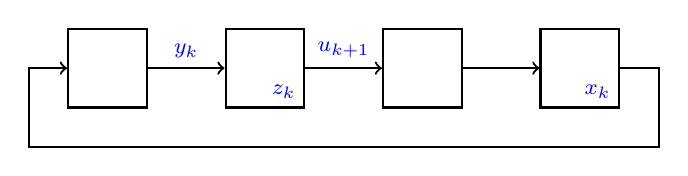
\begin{tikzpicture}
    % Blocks
    \node[draw, rectangle, minimum width = 1cm, minimum height = 1 cm, thick] (s) at (0,0) {$\sensor$};
    \node[draw, rectangle, minimum width = 1cm, minimum height = 1 cm, thick] (c) at (2,0) {$\ctrler$};
    \node[draw, rectangle, minimum width = 1cm, minimum height = 1 cm, thick] (a) at (4,0) {$\actuator$};
    \node[draw, rectangle, minimum width = 1cm, minimum height = 1 cm, thick] (p) at (6,0) {$\plant$};

    \node[anchor=south east, font=\footnotesize, blue] (z) at (c.south east) {$z_k$};
    \node[anchor=south east, font=\footnotesize, blue] (x) at (p.south east) {$x_k$};

    % Arrows
    \draw[->, thick] (s) -- node[above, blue, font=\footnotesize] {$y_k$} (c.west);
    \draw[->, thick] (c) -- node[above, blue, font=\footnotesize] {$u_{k+1}$} (a.west);
    \draw[->, thick] (a) -- (p.west);
    \draw[->, thick] (p.east) -| (7, -1) -| (-1, 0) -- (s.west);
\end{tikzpicture}
 
    \caption{Block diagram representing the interconnection of different components in a control system. The controller $\ctrler$ receives input from the sensor $\sensor$ and sends data to the actuator $\actuator$, which in turn acts on the plant $\plant$.}
    \label{fig:scheme}
\end{figure}
Starting from the \emph{sensors} $\sensor$, the plant is sampled at discrete time instants $k$.
The controller $\ctrler$ then polls the sensor channel for the latest sampled measurement signal to use in the calculation of the new control command $u_k$.
When the new control command is computed, the controller stores it in memory before sending it to the \emph{actuator} $\actuator$ at the beginning of the next control iteration.
Finally, the actuator acts upon the plant $\plant$, based on the command it received from the controller.

\subsection{Fault Model}%
\label{sec:impl}%
%
As anticipated, we aim at devising a stochastic analysis that determines the stability of the closed-loop system in the presence of faults.
We assume that three components in the real-time control system can experience faults (possibly simultaneously)
%
\begin{enumerate*}[label=(\roman*)]
    \item the \emph{sensor channel}, that transmits information between the sensor $\sensor$ and controller $\ctrler$,
    \item the \emph{control task}, that executes the algorithm of the controller $\ctrler$, and 
    \item the \emph{actuator channel}, that allows the controller $\ctrler$ to communicate with the actuator $\actuator$.
\end{enumerate*}
%
We provide a brief review of what can cause problems for both the controller and the input/output (IO) channels, together with some common implementation details.

\subsubsection*{Control Task and Overruns}
Controllers $\ctrler$ should periodically calculate a control signal based on~\eqref{eq:ctrler}. They are generally implemented in \emph{control tasks}, i.e., periodic tasks with implicit deadlines.
A typical implementation is the following.
\begin{lstlisting}[label=lst:control-job,caption={Typical control algorithm execution.}]
while True:
    y = read_sensor_ch()
    u, z = compute_control(y, z)
    sleep_until(next_activation)
    send_actuator_ch(u)
\end{lstlisting}
The code in Listing~\ref{lst:control-job} performs the following operations
\begin{enumerate*}[label=(\roman*)]
    \item it samples the current plant measurements in \texttt{y} using the sensor $\sensor$ (via the function \texttt{read\_sensor\_ch}),
    \item it calculates and stores in memory the next control signal \texttt{u} and the controller's updated state \texttt{z} (via \texttt{compute\_control}),
    \item it sleeps until the next activation (via \texttt{sleep\_until}), and
    \item it sends the control commands to the actuators $\actuator$ (via \texttt{send\_actuator\_ch}).
\end{enumerate*}

For the control task, each iteration of the loop in Listing~\ref{lst:control-job} is a new \emph{job}, and the $k$-th iteration corresponds to the job $j_k$.
The control job $j_k$ is \emph{released} at time $a_k = k\,\Ts$, where $\Ts$ is the \emph{period} of the control task.
The objective of each job is to complete its execution before its corresponding \emph{deadline} $d_k = a_k + \Ts = (k+1)\,\Ts$.
We denote with $f_k$ the time instant in which the control task \emph{completes} the execution of job $j_k$.
Ideally, $f_k \leq d_k$.

If $f_k > d_k$, job $j_k$ experiences an \emph{overrun}, or a deadline miss.
Overruns can be caused by many different factors, like preemption from higher priority tasks and interrupts~\cite{Stankovic:1995}, timeouts due to long wait times on the sensor channel~\cite{Ohlin:2006}, and cache misses that introduce delays in accessing the controller's stored variables~\cite{Wang:2012}.

Regardless of what caused the overrun, the scheduler needs to react.
In the literature~\cite{Cervin:2005}, mainly three simple \emph{deadline overrun strategies} have been considered
%
\begin{enumerate*}[label=(\roman*)]
    \item \tK{} -- i.e., \emph{killing} the job that overran its deadline (and releasing a new one), rolling back any (possibly partial) change performed by the job that missed its deadline, thus reverting the internal task state variables to their original value,
    \item \tS{} -- i.e., letting the job continue its execution, \emph{skipping} the subsequent job releases, until the current one has completed its execution, or
    \item \tQ{} -- i.e., combining the two, and letting the job continue its execution but at the same time \emph{queueing} the subsequent job executions.
\end{enumerate*}
%
In the case of \tS{} and \tQ{}, the job that continues executing operates on outdated data.
On the contrary, \tK{} allows the task to always work with fresh data, with the risk of throwing away near-completed computations.
The \tQ{} strategy has been shown to create chain effects which can severely damage control systems~\cite{Cervin:2005, Maggio:2020}, hence in this paper we only consider \tK{} and \tS{} as viable strategies.

\subsubsection*{Sensor Channel Dropouts}
Control systems rely on communication interfaces between the sensors/actuator and the controller code itself (i.e., the sensor and actuator channels).
A significant amount of research, including~\cite{Ling:2002, Linsenmayer:2017, Kauer:2014, Goswami:2014}, analysed the problem of control system's stability and performance when subject to sensor packet losses.
Losing packets over the sensor channel can lead to the controller not updating the control command, using old measurement data, or even missing job deadlines due to prolonged waiting times.
In these cases, the time in between two sampling instants is time-varying, and control design strategies can be applied to optimise the control system performance~\cite{Ghosh:2018, Schinkel:2002}.
However, this work does not take into account that packet losses could be combined with deadline overruns.

Furthermore, in the code snippet shown in Listing~\ref{lst:control-job}, there is no indication of how the control task reacts to sensor packet losses.
In classical controller implementations, if no sensor packet is received within a given time limit (typically a fraction of the deadline), the function \texttt{read\_sensor\_ch} \emph{times out}, and the control algorithm can perform one of the following two actions
%
\begin{enumerate*}[label=(\roman*)]
    \item \emph{continue} its execution, without updating the value of \texttt{y}, thus using the previous received sensor value, or
    \item \emph{avoid} executing the remaining instructions, terminating the computation early.
\end{enumerate*}

The choice of continuing or avoiding is highly dependent on the system dynamics.
Assuming that packet losses are relatively uncommon and the control period is typically short, using continue is advantageous.
In fact, if a packet is lost, it is still likely that the previous value reported by the sensor is a reasonable approximation of the physical environment.
We emphasise that continuing the execution is equivalent to the case when the controller does not directly poll the sensor channel, but rather reads the most recently received sensor value from memory (where it was stored by a receiver task).
On the other hand, avoiding the execution of the remaining instructions also prevents the controller from evolving its state \texttt{z} and control signal \texttt{u} in a possibly unsafe direction.
Listings~\ref{lst:continue} and~\ref{lst:pass} show more realistic versions of Listing~\ref{lst:control-job} for the continue and avoid cases.

\begin{lstlisting}[label=lst:continue,caption={Control code execution when the control computation is continued if the sensor reading function \texttt{read\_sensor\_ch} results in a timeout.}]
while True:
    y, tout_triggered = read_sensor_ch(tout_seconds)
    if tout_triggered:
        y = y_old
    u, z = compute_control(y, z)
    y_old = y
    sleep_until(next_activation)
    send_actuator_ch(u)
\end{lstlisting}
%
\newpage
\begin{lstlisting}[label=lst:pass,caption={Control code execution when the control computation is avoided if the sensor reading function \texttt{read\_sensor\_ch} results in a timeout.}]
while True:
    y, tout_triggered = read_sensor_ch(tout_seconds)
    if not tout_triggered:
        u, z = compute_control(y, z)
    sleep_until(next_activation)
    send_actuator_ch(u)
\end{lstlisting}

In Listings~\ref{lst:continue} and~\ref{lst:pass}, when \texttt{tout\_seconds} time units have passed without completion, the receive function \texttt{read\_sensor\_ch} sets the variable \texttt{tout\_triggered} to true.
In Listing~\ref{lst:continue}, the control algorithm continues executing its instructions using the old sensor value \texttt{y\_old}, i.e., the controller's internal state \texttt{z} will be updated and a new control command \texttt{u} will be sent to the actuators.
In Listing~\ref{lst:pass}, the control algorithm will not be run, i.e., the internal state \texttt{z} and the control command \texttt{u} are kept constant.

\subsubsection*{Actuator Channel Dropouts}
Packet losses on the actuator channel have not been studied as thoroughly as their sensor counterpart.
The reason likely comes from the fact that the actuator response is typically hardware-dependant and difficult to detect and compensate in the control algorithm.
If the actuator does not receive a new control command when it is expecting one, it defaults to a value dependent on the \emph{actuation mode}.
The actuation mode has received more attention, with different degradation or stabilising actuation policies being proposed~\cite{Ma:2018}.
However, the most common approaches involve either \tH{}ing the last received control command (i.e., $u_{k+1} = u_k$) or \tZ{}ing the output (i.e., $u_{k+1}=0$).
Similarly to choosing between continue and avoid, the choice of actuation mode is non-trivial and generally depend on the control system dynamic~\cite{Schenato:2009, Vreman:2021}.

\subsection{Problem Formulation}%
\label{sec:prob}%
Many different analysis frameworks have been proposed to evaluate the computational robustness to packet loss and deadline overruns of controllers~\cite{Ghosh:2018, Maggio:2020, Linsenmayer:2017, Heemels:2011}.
However, these analyses have two major shortcomings:
\begin{enumerate*}[label=(\roman*)]
    \item they are developed in isolation, and do not combine the presence of potential problems both in the computation and in the IO channels, and
    \item they rely on knowledge about the occurrence of events like deadline overruns or packet losses.
\end{enumerate*}
In fact, recent works on computational overruns~\cite{Maggio:2020, Linsenmayer:2017} rely on the weakly-hard task model~\cite{Bernat:2001} to constraint the sequence of deadline overruns; and recent work like~\cite{Ghosh:2018} are on the contrary working on the assumption that packet losses are detected and counteracted at the control level.
However, typical methods for deriving bounds on both packet losses and deadline overruns are probabilistic; for example, estimating the probability that a specific task in a system will overrun its deadline when a particular scheduling algorithm is employed~\cite{Chen:2019, Bruggen:2021}.

This paper aims at providing a control-theoretical analysis for how the closed-loop system robustness is affected by stochastic packet losses (on sensor and actuator channels), deadline overruns, and a combination thereof.
Furthermore, we want to devise an analysis method that benefits from the state-of-the-art results on fault occurrence estimation in real-time systems implementations~\cite{Chen:2019, Bruggen:2021}.
We assume to receive, as input, probabilities $p_c$, $p_s$, and $p_a$.
These represent respectively the probability of the control task missing its deadline, the probability of a failure on the sensor channel and the probability of a packet loss on the actuator channel.
The analysis provides -- as output -- a certificate that specifies that the system does or does not satisfy a stochastic stability requirement.
If the certificate verifies the stochastic stability of the closed-loop system, then the average value $\E{\tilde{x}_k}$ of the system state $\tilde{x}_k$, introduced in Equation~\eqref{eq:clsys}, converges to a given value and its standard deviation converges to zero.
This allows us to validate the control system implementation behaviour in the presence of undesirable faults.
